\chapter{集合函数与子集选择}
\label{chap:graph-set-functions}

在一片区域里安装传感器时，每个候选位置都能覆盖一块范围，但相邻位置的覆盖范围往往重叠。选定一组位置后，真正有意义的是这组位置合起来覆盖了多少，而不是各自覆盖面积的简单相加。同样，从一批特征里挑出一组、从一张图里挑出一部分顶点，评价的对象都是整组选择。前一章选择的是路径、生成树、流和匹配这些具有特定结构的对象；本章把候选对象放进一个有限的底集，研究怎样评价它的子集、怎样从累计评价中恢复各部分的贡献，以及怎样在数量或预算限制下选出好的子集。底集可以是图的顶点，也可以是边、特征或传感器，所以本章是从图向一般离散选择的扩展。

第~\ref{sec:graph-set-function-basics}节把“给子集赋值”写成集合函数，用二值向量表示子集，并用新增一个元素前后的评价差定义边际增益。第~\ref{sec:graph-set-function-properties}节依次区分单调性、模性与次模性：它们分别回答新增元素会不会降低评价、各元素的贡献是否固定、以及收益是否随已选集合增大而递减。第~\ref{sec:comb-cumulative-inversion}节转向另一项任务：已知每个子集的累计评价，怎样恢复每个子集自身的贡献；这一节只用有限求和与包含关系，不依赖前一节的性质。

后半章讨论选择。第~\ref{sec:graph-cardinality-selection}节在“至多选$k$个”的限制下逐轮加入边际增益最大的元素，并证明目标单调且次模时，这样得到的值不低于最优值的$1-(1-1/k)^k$倍。第~\ref{sec:graph-budget-selection}节让不同元素占用不同的预算，说明按单位成本选择怎样改进、又会在什么例子中失效。第~\ref{sec:graph-pairwise-binary-cut}节换成最小化问题：当目标只由一元项和满足一定条件的成对项组成时，它可以表示为割的容量，并用第~\ref{sec:graph-max-flow}节的最小割精确求解。这三节按约束与目标结构分别组织，彼此不是一条必然的依赖链。

% 第4章第1节：集合函数（集合函数的定义；子集与二值向量；边际增益）。

\section{集合函数}
\label{sec:graph-set-function-basics}

给每个元素赋一个数，只需要一张长度为元素个数的表；给每个子集赋一个数，则要考虑元素之间怎样相互影响。本节先用传感器覆盖说明为什么需要以子集为自变量的函数，再把子集写成二值向量，最后定义新增一个元素带来的评价变化。这三样东西是后面判断函数性质、设计选择方法时共同使用的记号。

\subsection{集合函数的定义}
\label{sec:graph-setfn-definition}

\paragraph{传感器覆盖实例}
图~\ref{fig:graph-setfn-sensor-coverage}是一块由上下两行、左右八列组成的区域，共$16$个格子。有四个候选传感器：$a$覆盖第$2$至$6$列的$10$个格子，$b$覆盖第$1$至$4$列的$8$个格子，$c$覆盖第$5$至$8$列的$8$个格子，$d$只覆盖左上角的$1$个格子。选定一组传感器后，我们关心这组传感器合起来覆盖了多少个不同的格子。记传感器$v$覆盖的格子集合为$C_v$，选定的传感器集合为$S$，覆盖量就是
\[
  F(S)=\Bigl|\bigcup_{v\in S}C_v\Bigr|.
\]
单独看，$F(\{a\})=10$，$F(\{b\})=8$；两者一起时，第$2$至$4$列被重复覆盖，$F(\{a,b\})=12$，而不是$10+8=18$。整组的价值不能由各成员的价值相加得到，因此评价必须直接以“哪些传感器被选中”为输入。本章后面几节都用这个实例做算例。

\begin{figure}[!htb]
  \centering
  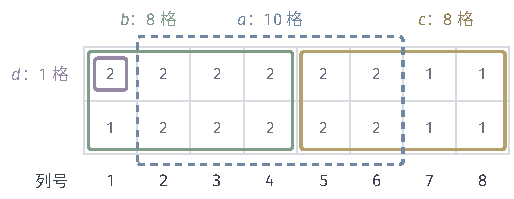
\includegraphics[width=87.027mm]{figures/01-basic-mathematics/04-graphs/tikz/c4-sensor-coverage/figure.pdf}
  \caption{贯穿本章的传感器覆盖实例。区域由$2\times 8$个格子组成；绿色框为$b$（第$1$至$4$列），黄色框为$c$（第$5$至$8$列），蓝色虚线框为$a$（第$2$至$6$列），紫色小框为$d$（左上角一格）。格内数字是覆盖该格的传感器个数，数字$2$所在的格子都被重复覆盖，因而各传感器覆盖格数之和大于它们合起来覆盖的格数。}
  \label{fig:graph-setfn-sensor-coverage}
\end{figure}

覆盖量的输入是一个子集，输出是一个实数。把这种对应一般化，就得到下面的定义。

\begin{definition}[集合函数]
\label{def:graph-setfn-set-function}
设$V$是有限集合，称为\term{底集}（ground set）。把$V$的每个子集对应到一个实数的映射
\[
  F:\mathcal P(V)\to\mathbb R
\]
称为$V$上的\term{集合函数}（set function），其中$\mathcal P(V)$是$V$的幂集。
\end{definition}

定义要求$F$在每个子集上都有值，包括空集。空集表示“什么都不选”，它的值是比较其他选择的起点：覆盖量取$F(\varnothing)=0$，一个带固定开销的评价则可能取非零值。底集中的元素可以是传感器、特征、顶点或边；集合函数本身并不要求底集带有图结构。

\paragraph{三个例子}
同一个子集可以按不同目的评价。以传感器实例为例，给四个传感器分别指定安装成本$4,3,4,1$（依次对应$a,b,c,d$），总成本
\[
  c(S)=\sum_{v\in S}c_v
\]
是一个集合函数，例如$c(\{a,b\})=7$；覆盖量$F$是另一个集合函数，$F(\{a,b\})=12$。第三个例子来自图。设$\mathcal G=(V,E)$是无向图，每条边$\{i,j\}$带非负权$w_{i,j}$。顶点子集$S$把顶点分成$S$与$V\setminus S$两侧，这正是第~\ref{sec:graph-minimum-spanning-tree}节所说的割；两端分居两侧的边的权之和
\[
  \operatorname{cut}(S)=\sum_{\{i,j\}\in E:\ |\{i,j\}\cap S|=1}w_{i,j}
\]
称为$S$的割权。这里的底集是顶点集，$\operatorname{cut}$以顶点子集为自变量。三个例子分别累计单项成本、合并覆盖范围和统计跨越两侧的边，元素之间的相互影响各不相同，下一节将据此区分它们的性质。

\paragraph{取值表与求值规则}
由式~\eqref{eq:comb-power-set-count}，$n$元底集有$2^n$个子集，所以一个集合函数的完整取值表有$2^n$项。传感器实例只有$16$项，可以全部写出；底集有$50$个元素时，取值表已超过$10^{15}$项，无法存储。实际问题中的集合函数通常由一条规则给出：给定$S$，按规则算出$F(S)$。覆盖量的规则是求并集再计数，割权的规则是扫描全部边。这样的一次计算称为一次\emph{求值}，它的代价取决于具体表示：覆盖量的一次求值要处理$S$中各传感器的覆盖范围，割权的一次求值要检查每条边。后面分析算法时，我们把求值次数和每次求值的代价分开计算，不把求值默认视为免费。

\subsection{子集与二值向量}
\label{sec:graph-setfn-binary-vectors}

给底集的元素固定编号$V=\{1,\ldots,n\}$。第~\ref{sec:comb-ordered-unordered}节已经说明，子集$S$与零一记录一一对应。把这条记录写成向量$\bm x=(x_1,\ldots,x_n)\in\{0,1\}^n$，其中
\[
  x_i=\mathbb I\{i\in S\},
\]
称$\bm x$为$S$的\term{指示向量}（indicator vector）。反过来，由$\bm x$恢复子集只需收集取值为$1$的坐标：$S=\{i:x_i=1\}$。

集合运算在指示向量上逐坐标进行。设$S,T$的指示向量为$\bm x,\bm y$，则元素个数是坐标之和，$|S|=\sum_ix_i$；并集的第$i$个坐标是$\max\{x_i,y_i\}$，交集的第$i$个坐标是$\min\{x_i,y_i\}=x_iy_i$，补集的第$i$个坐标是$1-x_i$。包含关系$S\subseteq T$对应逐坐标的$x_i\leq y_i$。

于是集合函数也可以写成二值向量的函数：令$f(\bm x)=F(\{i:x_i=1\})$，$f$与$F$只是同一组数值的两种索引方式。图~\ref{fig:graph-setfn-subset-binary-cube}以三元底集为例画出这一对应：八个子集恰好是立方体的八个顶点，立方体的每条边连接只差一个元素的两个子集，也就是只差一个坐标的两个向量。

\begin{figure}[!htb]
  \centering
  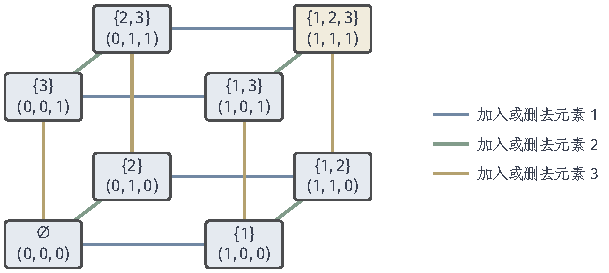
\includegraphics[width=103.209mm]{figures/01-basic-mathematics/04-graphs/tikz/c4-subset-binary-cube/figure.pdf}
  \caption{三元底集$V=\{1,2,3\}$的八个子集与指示向量$(x_1,x_2,x_3)$排成立方体的顶点。每个框上行是子集，下行是对应的向量；边的颜色表示沿这条边加入或删去哪个元素，也就是改变哪个坐标。沿任一条边向上走一步，就是在当前子集中加入一个元素。}
  \label{fig:graph-setfn-subset-binary-cube}
\end{figure}

这一改写只换了表示方式，并没有带来额外结构。写成$f(\bm x)$之后，$f$不一定是各坐标的函数之和，也不一定能分解成只读取少数坐标的局部项；在$\{0,1\}^n$上谈连续性或求导也没有意义。第~\ref{sec:graph-pairwise-binary-cut}节和第~\ref{chap:graph-dynamic-programming}章讨论的，正是函数确实具有某种局部分解时可以怎样利用它。

\subsection{边际增益}
\label{sec:graph-setfn-marginal-gain}

选择子集时，最直接的问题是：在已经选好的集合上再加一个元素，评价会改变多少。

\begin{definition}[边际增益]
\label{def:graph-setfn-marginal-gain}
设$F$是$V$上的集合函数，$S\subseteq V$，$v\in V\setminus S$。称
\[
  \Delta(v\mid S)=F(S\cup\{v\})-F(S)
\]
为元素$v$相对于集合$S$的\term{边际增益}（marginal gain）。
\end{definition}

边际增益同时依赖新元素和已选集合。图~\ref{fig:graph-setfn-marginal-gain-overlap}比较同一个传感器$c$在两种情况下的增益：从空集加入时，$c$的$8$个格子都是新覆盖的，$\Delta(c\mid\varnothing)=8$；已经选了$a$之后，$c$的第$5$、$6$列已被$a$覆盖，只有第$7$、$8$列的$4$个格子是新的，$\Delta(c\mid\{a\})=4$。所以谈论一个元素“值多少”时，必须说明是相对于哪个已选集合。

\begin{figure}[!htb]
  \centering
  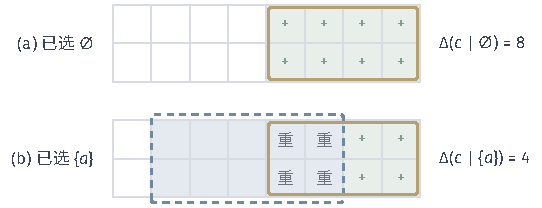
\includegraphics[width=91.74mm]{figures/01-basic-mathematics/04-graphs/tikz/c4-marginal-gain-overlap/figure.pdf}
  \caption{同一传感器$c$（黄色框）的边际增益随已选集合变化。(a) 已选集合为空，$c$覆盖的$8$个格子（绿色，标“$+$”）全部是新覆盖；(b) 已选$\{a\}$（蓝色底与蓝色虚线框），$c$与$a$重叠的第$5$、$6$列（标“重”）不再计数，只有第$7$、$8$列的$4$个格子是新覆盖。}
  \label{fig:graph-setfn-marginal-gain-overlap}
\end{figure}

\paragraph{逐个加入的累计}
把一个集合的元素逐个加入，函数的总变化就是一串边际增益之和。设$A\subseteq B\subseteq V$，把$B\setminus A$中的元素按任意次序排成$v_1,\ldots,v_r$，记$A_0=A$，$A_k=A\cup\{v_1,\ldots,v_k\}$。于是$A_r=B$，并且
\begin{equation}
  F(B)-F(A)=\sum_{k=1}^{r}\bigl(F(A_k)-F(A_{k-1})\bigr)=\sum_{k=1}^{r}\Delta(v_k\mid A_{k-1}).
  \label{eq:graph-setfn-telescoping}
\end{equation}
第一个等号是裂项求和（式~\eqref{eq:prelim-telescoping-sum}）：中间的$F(A_1),\ldots,F(A_{r-1})$各出现一次正号、一次负号而抵消。第二个等号是因为$A_k=A_{k-1}\cup\{v_k\}$且$v_k\notin A_{k-1}$。

在传感器实例中取$A=\varnothing$、$B=\{a,b,c\}$。按$a,c,b$的次序加入，三个增益依次是$10,4,2$；按$b,c,a$的次序加入，三个增益依次是$8,8,0$。两种次序的总和都是$F(\{a,b,c\})=16$，但每一步的增益随次序改变。式~\eqref{eq:graph-setfn-telescoping}是下一节判别性质和第~\ref{sec:graph-cardinality-selection}节分析贪心算法的共同工具。

边际增益只描述一步的变化。在空集上，$a$的增益$10$是四个传感器中最大的，但只能选两个传感器时，最好的组合是$\{b,c\}$，它覆盖全部$16$个格子，并不包含$a$。单步增益大，不保证这一步属于某个全局最优子集；这一点将在第~\ref{sec:graph-cardinality-selection}节具体比较。

% 第4章第2节：集合函数的性质（单调性；模性；次模性与超模性）。

\section{集合函数的性质}
\label{sec:graph-set-function-properties}

上一节的三个例子在“加入一个元素会怎样改变评价”这个问题上表现不同：加入传感器不会减少覆盖，但可能增加的覆盖越来越少；加入一项成本总是增加固定的数额；把一个顶点移到$S$一侧，割权可能增加也可能减少。本节把这些表现分别写成单调性、模性和次模性，并说明三者各有条件，不能互相推出。

\subsection{单调性}
\label{sec:graph-setfn-monotonicity}

多装一个传感器，覆盖的格子只会增加或保持不变。把这一性质写成子集之间的比较，就是下面的定义。

\begin{definition}[单调非减]
\label{def:graph-setfn-monotone}
若对任意$A\subseteq B\subseteq V$都有$F(A)\leq F(B)$，称集合函数$F$\term{单调非减}（monotone nondecreasing），简称单调。
\end{definition}

定义比较的是任意两个有包含关系的子集，检查起来要考虑很多对。借助式~\eqref{eq:graph-setfn-telescoping}，它可以化成只检查单个元素的条件：$F$单调，当且仅当对每个$S\subseteq V$和每个$v\notin S$都有$\Delta(v\mid S)\geq0$。必要性只需取$A=S$、$B=S\cup\{v\}$。充分性：对任意$A\subseteq B$，式~\eqref{eq:graph-setfn-telescoping}把$F(B)-F(A)$写成若干个边际增益之和，每一项都非负，所以$F(A)\leq F(B)$。

覆盖量是单调的：加入$v$后新增的格子数$\Delta(v\mid S)=|C_v\setminus\bigcup_{u\in S}C_u|$不会是负数。

\paragraph{单调性与非负性的区别}
覆盖量含在一个目标里，并不保证整个目标单调。把覆盖量减去安装成本，得到净收益$G(S)=F(S)-c(S)$。$G(\{b\})=8-3=5$，而$G(\{b,d\})=8-4=4$：$d$覆盖的那一格已被$b$覆盖，加入$d$不增加覆盖，却多花$1$个单位成本，所以净收益下降。

函数值全为非负，也不能推出单调。在二元底集$\{1,2\}$上取
\[
  F(\varnothing)=1,\quad F(\{1\})=3,\quad F(\{2\})=2,\quad F(\{1,2\})=2,
\]
四个值都是正数，但$\Delta(2\mid\{1\})=2-3=-1<0$。反过来，单调也不能推出$F(\varnothing)=0$：常数函数$F\equiv5$是单调的。$F(\varnothing)=0$称为\emph{归一化}，它是一项约定；对任意集合函数，减去常数$F(\varnothing)$就得到归一化的函数，而所有边际增益保持不变。归一化且单调的函数必然处处非负，因为$F(S)\geq F(\varnothing)=0$。

\subsection{模性}
\label{sec:graph-setfn-modularity}

总成本$c(S)$具有最简单的结构：每个元素贡献一个固定的数，彼此互不影响。一般地，取常数$c_0$和每个元素的权$w_v$，令
\begin{equation}
  F(S)=c_0+\sum_{v\in S}w_v .
  \label{eq:graph-setfn-modular-form}
\end{equation}
这时对任意$S$和$v\notin S$，$\Delta(v\mid S)=w_v$，增益与已选集合无关。由上一小节的判别条件，这样的$F$单调当且仅当每个$w_v\geq0$；常数$c_0$不影响任何边际增益。

\paragraph{模等式}
对形如式~\eqref{eq:graph-setfn-modular-form}的函数和任意两个子集$A,B$，比较$F(A)+F(B)$与$F(A\cup B)+F(A\cap B)$。两边都含两个常数$c_0$。对一个元素$v$：若$v$同时属于$A$和$B$，则$w_v$在左边计两次，在右边的并集与交集中也各计一次；若$v$只属于其中一个，则$w_v$在两边都只计一次；若$v$都不属于，则两边都不计。所以
\begin{equation}
  F(A)+F(B)=F(A\cup B)+F(A\cap B).
  \label{eq:graph-setfn-modular-equality}
\end{equation}
对所有$A,B\subseteq V$满足式~\eqref{eq:graph-setfn-modular-equality}的集合函数称为\term{模函数}（modular function）。

反过来，模等式也足以恢复固定权重的表示，因此它可以用来判断元素之间有没有交互。设$F$是模函数，取$S\neq\varnothing$与$v\in S$，在式~\eqref{eq:graph-setfn-modular-equality}中令$A=S\setminus\{v\}$、$B=\{v\}$，这时$A\cup B=S$，$A\cap B=\varnothing$，得到
\[
  F(S)=F(S\setminus\{v\})+\bigl(F(\{v\})-F(\varnothing)\bigr).
\]
对$|S|$归纳，就得到$F(S)=F(\varnothing)+\sum_{v\in S}\bigl(F(\{v\})-F(\varnothing)\bigr)$，即式~\eqref{eq:graph-setfn-modular-form}取$c_0=F(\varnothing)$、$w_v=F(\{v\})-F(\varnothing)$。覆盖量不是模函数：$F(\{a\})+F(\{b\})=18$，而$F(\{a,b\})+F(\varnothing)=12$，差值$6$正是两者重叠的格子数。

\subsection{次模性}
\label{sec:graph-setfn-submodularity}

覆盖量的增益随已选集合增大而变小：已覆盖的格子越多，新传感器能补上的格子越少。图~\ref{fig:graph-setfn-marginal-gain-overlap}中，$\Delta(c\mid\varnothing)=8$，$\Delta(c\mid\{a\})=4$；再加入$b$之后，$\Delta(c\mid\{a,b\})=4$，没有继续变小，但也没有变大。把“不会变大”作为要求，就得到边际收益递减的条件。

\begin{definition}[次模函数]
\label{def:graph-setfn-submodular}
若对任意$A\subseteq B\subseteq V$和任意$v\in V\setminus B$都有
\begin{equation}
  \Delta(v\mid A)\geq\Delta(v\mid B),
  \label{eq:graph-setfn-diminishing-returns}
\end{equation}
称集合函数$F$是\term{次模}函数（submodular function）。
\end{definition}

条件中的$v$不属于$B$，从而也不属于$A$，两个增益都有定义。次模性还有一种不出现边际增益的写法，它和模等式形式相同，只是把等号换成不等号。

\begin{theorem}[次模性的两种刻画]
\label{thm:graph-setfn-submodular-equivalence}
设$V$是有限集合，$F$是$V$上的集合函数。$F$满足式~\eqref{eq:graph-setfn-diminishing-returns}，当且仅当对任意$X,Y\subseteq V$都有
\begin{equation}
  F(X)+F(Y)\geq F(X\cup Y)+F(X\cap Y).
  \label{eq:graph-setfn-submodular-inequality}
\end{equation}
\end{theorem}

\begin{proof}
先设式~\eqref{eq:graph-setfn-submodular-inequality}成立。给定$A\subseteq B$和$v\notin B$，取$X=A\cup\{v\}$、$Y=B$。由$A\subseteq B$得$X\cup Y=B\cup\{v\}$；由$v\notin B$得$X\cap Y=A$。代入式~\eqref{eq:graph-setfn-submodular-inequality}，
\[
  F(A\cup\{v\})+F(B)\geq F(B\cup\{v\})+F(A),
\]
移项即$\Delta(v\mid A)\geq\Delta(v\mid B)$。

再设式~\eqref{eq:graph-setfn-diminishing-returns}成立。给定$X,Y$，记$C=X\cap Y$，把$Y\setminus X$中的元素按任意次序排成$y_1,\ldots,y_r$。分别从$X$和从$C$出发逐个加入这些元素，由式~\eqref{eq:graph-setfn-telescoping}，
\[
  \begin{gathered}
  F(X\cup Y)-F(X)=\sum_{k=1}^{r}\Delta\bigl(y_k\mid X\cup\{y_1,\ldots,y_{k-1}\}\bigr),\\
  F(Y)-F(C)=\sum_{k=1}^{r}\Delta\bigl(y_k\mid C\cup\{y_1,\ldots,y_{k-1}\}\bigr).
  \end{gathered}
\]
这里用到$X\cup(Y\setminus X)=X\cup Y$与$C\cup(Y\setminus X)=Y$。对每个$k$，$C\cup\{y_1,\ldots,y_{k-1}\}\subseteq X\cup\{y_1,\ldots,y_{k-1}\}$，且$y_k$不属于后者（$y_k\notin X$，并且与前面的$y_j$不同）。由式~\eqref{eq:graph-setfn-diminishing-returns}，第二个和的每一项不小于第一个和的对应项，所以$F(X\cup Y)-F(X)\leq F(Y)-F(C)$，移项即得式~\eqref{eq:graph-setfn-submodular-inequality}。
\end{proof}

两种刻画各有用处：式~\eqref{eq:graph-setfn-diminishing-returns}直接对应“收益递减”的直观，适合分析逐个加入元素的算法；式~\eqref{eq:graph-setfn-submodular-inequality}只涉及四个函数值，适合验证具体函数。模函数在式~\eqref{eq:graph-setfn-submodular-inequality}中处处取等号，所以模函数是次模的。

\paragraph{覆盖量是次模的}
设$A\subseteq B$，$v\notin B$。$v$相对于$S$的增益是$C_v$中尚未被$S$覆盖的格子数，即$\Delta(v\mid S)=|C_v\setminus U(S)|$，其中$U(S)=\bigcup_{u\in S}C_u$。由$A\subseteq B$得$U(A)\subseteq U(B)$，于是$C_v\setminus U(B)\subseteq C_v\setminus U(A)$，取元素个数就得到式~\eqref{eq:graph-setfn-diminishing-returns}。这个论证不依赖格子的具体排列，所以任何“覆盖了多少个不同对象”的函数都是次模的，称为\term{覆盖函数}（coverage function）。

\paragraph{割权是次模的}
割权按边累加，所以先看一条权为$w$的边$\{i,j\}$单独贡献的函数：它在$S$恰含$i,j$之一时取$w$，否则取$0$。对不是端点的元素，这条边的贡献不随它的加入而改变，增益为$0$。加入端点$i$时，若$j$已在集合中，这条边从跨越两侧变为两端同侧，增益为$-w$；若$j$不在集合中，这条边从两端同侧变为跨越两侧，增益为$+w$。

现在取$A\subseteq B$、$i\notin B$，按$j$的归属分三种情形比较两个增益，见图~\ref{fig:graph-setfn-cut-submodular-cases}。若$j\in A$，则$j$也在$B$中，两个增益都是$-w$；若$j\in B\setminus A$，则$\Delta(i\mid A)=+w$而$\Delta(i\mid B)=-w$；若$j\notin B$，两个增益都是$+w$。三种情形都满足$\Delta(i\mid A)\geq\Delta(i\mid B)$，所以单条边的贡献是次模的。若干个函数各自满足式~\eqref{eq:graph-setfn-diminishing-returns}时，把这些不等式逐项相加，可知它们的和也满足，于是$\operatorname{cut}$作为各边贡献之和也是次模的。边权非负在这里是必要的：若某条边的权为负，第二种情形的不等号就反向了。

\begin{figure}[!htb]
  \centering
  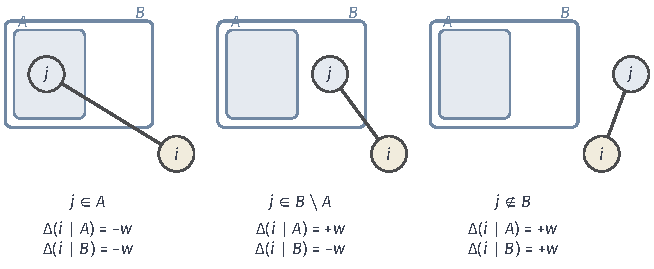
\includegraphics[width=110.723mm]{figures/01-basic-mathematics/04-graphs/tikz/c4-cut-submodular-cases/figure.pdf}
  \caption{割权函数次模性的逐边验证。固定一条权为$w\geq0$的边$\{i,j\}$，已选集合$A\subseteq B$（内框为$A$，外框为$B$），待加入的端点$i$（黄色）不在$B$中。按另一端点$j$的位置分三种情形：$j\in A$时两个增益都是$-w$；$j\in B\setminus A$时$A$上增益为$+w$、$B$上增益为$-w$；$j\notin B$时两个增益都是$+w$。每种情形都有$\Delta(i\mid A)\geq\Delta(i\mid B)$。}
  \label{fig:graph-setfn-cut-submodular-cases}
\end{figure}

\paragraph{次模与单调互不蕴含}
割权常常随集合增大而下降：$\operatorname{cut}(\varnothing)=\operatorname{cut}(V)=0$，而中间的子集可以有正的割权。图~\ref{fig:graph-setfn-property-counterexamples}(b)是只有一条权$1$的边的情形，割权依次为$0,1,1,0$，从单元素集到$\{1,2\}$时下降，所以次模函数不必单调。反方向，图~\ref{fig:graph-setfn-property-counterexamples}(a)的函数
\[
  F(S)=\max\bigl\{3\,\mathbb I\{\{1,2\}\subseteq S\},\ \mathbb I\{3\in S\}\bigr\}
\]
是单调的，但$\Delta(2\mid\varnothing)=0<3=\Delta(2\mid\{1\})$，违反式~\eqref{eq:graph-setfn-diminishing-returns}，所以单调函数也不必次模。

\begin{figure}[!htb]
  \centering
  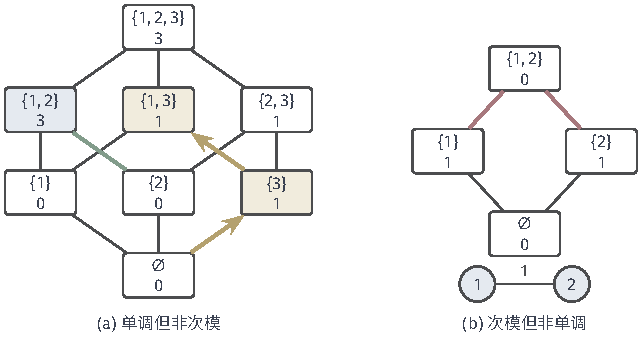
\includegraphics[width=108.687mm]{figures/01-basic-mathematics/04-graphs/tikz/c4-property-counterexamples/figure.pdf}
  \caption{单调性与次模性互不蕴含。每个框上行是子集，下行是函数值，连线连接只差一个元素的子集。(a) $F(S)=\max\{3\,\mathbb I\{\{1,2\}\subseteq S\},\mathbb I\{3\in S\}\}$：沿任一连线向上函数值不减，但绿色连线$\{2\}\to\{1,2\}$的增益$3$大于从空集加入$2$的增益$0$；黄色箭头是第~\ref{sec:graph-cardinality-selection}节贪心选择的路径，蓝色框是两元素时的最优集合。(b) 单条权$1$的边上的割权：次模，但红色连线上函数值从$1$降到$0$。}
  \label{fig:graph-setfn-property-counterexamples}
\end{figure}

\paragraph{超模性与协同}
把式~\eqref{eq:graph-setfn-diminishing-returns}的不等号反过来，即要求$\Delta(v\mid A)\leq\Delta(v\mid B)$，得到的函数称为\term{超模}函数（supermodular function）；等价地，$F$超模当且仅当$-F$次模。超模描述的是协同：两个部件只有同时具备才能工作时，单独加入任何一个的增益都是$0$，在另一个已经存在时加入，增益才是正的。例如$F(S)=\mathbb I\{\{1,2\}\subseteq S\}$是超模的。图~\ref{fig:graph-setfn-property-counterexamples}(a)的函数既不是次模也不是超模：元素$1,2$之间是协同的，而元素$3$与$\{1,2\}$之间是替代的，$\Delta(3\mid\varnothing)=1>0=\Delta(3\mid\{1,2\})$。

单调、模、次模、超模分别约束不同的东西，覆盖量、割权、净收益和上面的反例说明它们可以以各种方式组合出现。后面各节的算法保证都会同时写明目标是最大化还是最小化、函数是否单调、是否次模，以及约束是什么；只凭“次模”二字，并不能决定应当采用哪种方法。

% 第4章第3节：子集累计与 Möbius 反演（子集格与累计；Möbius 反演；反演的计算与算例；有限偏序集上的推广）。

\section{子集累计与 Möbius 反演}
\label{sec:comb-cumulative-inversion}

本节转向另一类问题。设想每个课程组合有一个总得分：单门课各有自己的贡献，某两门课同时选又会产生额外的配合效果，配合也可能是负的。我们能观察到的是每个组合的总得分，想知道的却是每个组合\emph{自身}贡献了多少。第~\ref{sec:comb-overlap-counting}节的容斥原理由各交集的大小恢复并集的大小，这里要做的是同一类“由累计量恢复局部量”的事，只是对象换成了一般的数值。本节只用有限求和与包含关系，不依赖上一节的单调或次模假设，也不是后面选择算法的前提。

\subsection{子集格与累计}
\label{sec:graph-setfn-subset-lattice}

累计沿包含关系进行，所以先把包含关系画出来。第~\ref{sec:prelim-order-relations}节已经说明，包含关系是幂集上的偏序。有限集合$V$的全部子集连同包含关系称为$V$的\term{子集格}（subset lattice）：两个子集的交是它们最大的公共子集，并是包含两者的最小集合。图~\ref{fig:comb-mobius-cumulative-local}按元素个数自下而上分层画出$V_0=\{1,2,3,4\}$的子集格，每条连线连接只差一个元素的两个子集，沿连线向上一步就是加入一个元素。图~\ref{fig:graph-setfn-subset-binary-cube}中的立方体正是三元底集的子集格。

从$S$出发沿连线一路向下能到达的子集，恰好是$S$的全部子集。例如从$\{1,3\}$向下只能到达$\{1\}$、$\{3\}$和空集。下面定义的累计值，正是沿这些向下的路径收集贡献。

\begin{figure}[!htb]
  \centering
  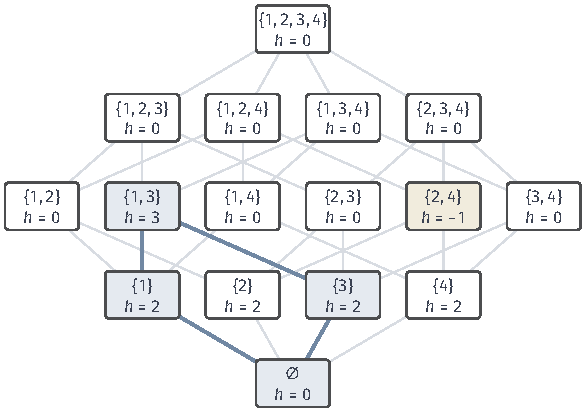
\includegraphics[width=99.187mm]{figures/01-basic-mathematics/04-graphs/tikz/c4-subset-lattice-cumulative/figure.pdf}
  \caption{四元素集合$V_0=\{1,2,3,4\}$的子集格与各子集自身的贡献$h$。子集按元素个数自下而上分层，连线连接只差一个元素的两个子集；框内上行为子集，下行为教学设定的贡献。蓝色标出$\{1,3\}$及其全部子集，它们的贡献相加得到累计值$g(\{1,3\})=0+2+2+3=7$；黄色框$\{2,4\}$的自身贡献为负。}
  \label{fig:comb-mobius-cumulative-local}
\end{figure}

\paragraph{自身贡献与累计值}
给每个子集$T$指定一个实数$h(T)$，表示$T$作为整体\emph{自身}带来的贡献：单元素集的贡献是单门课的得分，二元集的贡献是两门课的配合效果，依此类推。$S$的累计值收集它的全部子集的贡献：
\begin{equation}
  g(S)=\sum_{T\subseteq S}h(T).
  \label{eq:comb-zeta-transform}
\end{equation}
$g$与$h$都是$V$上的集合函数。注意累计不只相加单元素的贡献，$S$内部更大子集的配合贡献也计入其中。

图~\ref{fig:comb-mobius-cumulative-local}的教学设定让四个单项各贡献$2$，$\{1,3\}$另有配合贡献$3$，$\{2,4\}$另有配合贡献$-1$，其余子集（包括空集和全部三元、四元子集）的贡献为$0$。于是
\[
  g(\{1,3\})=h(\varnothing)+h(\{1\})+h(\{3\})+h(\{1,3\})=0+2+2+3=7,
\]
而两个单项的累计值之和只有$g(\{1\})+g(\{3\})=4$，多出的$3$正是$\{1,3\}$自身的贡献。反演要回答相反方向的问题：只知道每个子集的累计值$g$，怎样读出每个子集自身的贡献$h$。

\subsection{Möbius 反演}
\label{sec:graph-setfn-mobius-inversion}

先看两元素的情形。$g(\{1,3\})$包含$h(\varnothing)$、$h(\{1\})$、$h(\{3\})$和$h(\{1,3\})$四项。减去$g(\{1\})=h(\varnothing)+h(\{1\})$和$g(\{3\})=h(\varnothing)+h(\{3\})$，两个单项贡献被去掉，但$h(\varnothing)$被多减了一次，再加回$g(\varnothing)=h(\varnothing)$，剩下的恰是
\[
  h(\{1,3\})=g(\{1,3\})-g(\{1\})-g(\{3\})+g(\varnothing).
\]
符号按子集比$S$少几个元素交替变化。一般情形的公式正是这样，称为\term{Möbius反演}（Möbius inversion）。

\begin{theorem}[子集格上的 Möbius 反演]
\label{thm:comb-mobius-inversion}
设$V$为有限集合，$g,h:\mathcal P(V)\to\mathbb R$。若对每个$S\subseteq V$式~\eqref{eq:comb-zeta-transform}成立，则对每个$S\subseteq V$有
\begin{equation}
  h(S)=\sum_{T\subseteq S}(-1)^{|S|-|T|}g(T).
  \label{eq:comb-mobius-inversion}
\end{equation}
反过来，若对每个$S$式~\eqref{eq:comb-mobius-inversion}成立，则式~\eqref{eq:comb-zeta-transform}也对每个$S$成立。
\end{theorem}

\begin{proof}
把式~\eqref{eq:comb-zeta-transform}代入式~\eqref{eq:comb-mobius-inversion}右侧，得到对全部满足$R\subseteq T\subseteq S$的集合对$(R,T)$的双重和。先固定$T$再取$R$，与先固定$R$再取$T$，遍历的是同一批集合对，所以可以像第~\ref{sec:prelim-finite-sums-products}节的三角形求和那样交换有限求和的次序：
\[
  \sum_{T\subseteq S}(-1)^{|S|-|T|}\sum_{R\subseteq T}h(R)
  =\sum_{R\subseteq S}h(R)\sum_{T:\,R\subseteq T\subseteq S}(-1)^{|S|-|T|}.
\]
固定$R$后，满足$R\subseteq T\subseteq S$的$T$由$S\setminus R$中哪些元素被加入决定，即$T=R\cup D$，$D\subseteq S\setminus R$任意，且$|S|-|T|=|S\setminus R|-|D|$。记$q=|S\setminus R|$，按$|D|=j$分组，大小为$j$的$D$有$\binom qj$个，所以内层和等于
\[
  \sum_{j=0}^{q}\binom qj(-1)^{q-j}=(-1)^q\sum_{j=0}^{q}(-1)^j\binom qj
  =\begin{cases}1,&q=0,\\0,&q\geq1,\end{cases}
\]
最后一步用式~\eqref{eq:comb-alternating-subset-count}。内层和只在$R=S$时为$1$，在$R$是$S$的真子集时为$0$，所以真子集上的贡献全部抵消，右侧只剩$h(S)$。

反方向同样直接核对。由式~\eqref{eq:comb-mobius-inversion}给出$h$，代入$\sum_{T\subseteq S}h(T)$并交换求和次序，
\[
  \sum_{T\subseteq S}h(T)=\sum_{R\subseteq S}g(R)\sum_{T:\,R\subseteq T\subseteq S}(-1)^{|T|-|R|}.
\]
仍写$T=R\cup D$，内层和等于$\sum_{j=0}^{q}(-1)^j\binom qj$，它在$R=S$时只有$D=\varnothing$一项而等于$1$，在$R\neq S$时为$0$。所以右侧等于$g(S)$。
\end{proof}

定理说明式~\eqref{eq:comb-zeta-transform}与式~\eqref{eq:comb-mobius-inversion}是一对互逆的变换：从贡献到累计，再从累计回到贡献，不丢失任何信息。证明中起作用的是组合数的交错和为零，这与容斥原理的证明相同。区别在于，容斥最终使并集中的每个元素恰计一次，反演最终只保留指定子集自身的贡献。

\subsection{反演的计算与算例}
\label{sec:graph-setfn-mobius-computation}

\paragraph{四元素算例}
记$\mathbb I\{\cdot\}$为条件成立时取$1$、否则取$0$的指示函数。沿用图~\ref{fig:comb-mobius-cumulative-local}的设定，累计值可以写成
\[
  g(S)=2|S|+3\,\mathbb I\{\{1,3\}\subseteq S\}-\mathbb I\{\{2,4\}\subseteq S\}.
\]
其中$2|S|$收集$S$中各单项的贡献，后两项在$S$包含$\{1,3\}$或$\{2,4\}$时计入相应的配合贡献。表~\ref{tab:comb-four-element-mobius}列出全部$16$个累计值，以及只用这些累计值按式~\eqref{eq:comb-mobius-inversion}恢复的贡献。

\begin{table}[!htb]
  \centering
  \begin{tabular}{ccc@{\qquad}ccc}
    \toprule
    $S$ & $g(S)$ & $h(S)$ & $S$ & $g(S)$ & $h(S)$ \\
    \midrule
    $\varnothing$ & $0$ & $0$ & $\{2,3\}$ & $4$ & $0$ \\
    $\{1\}$ & $2$ & $2$ & $\{2,4\}$ & $3$ & $-1$ \\
    $\{2\}$ & $2$ & $2$ & $\{3,4\}$ & $4$ & $0$ \\
    $\{3\}$ & $2$ & $2$ & $\{1,2,3\}$ & $9$ & $0$ \\
    $\{4\}$ & $2$ & $2$ & $\{1,2,4\}$ & $5$ & $0$ \\
    $\{1,2\}$ & $4$ & $0$ & $\{1,3,4\}$ & $9$ & $0$ \\
    $\{1,3\}$ & $7$ & $3$ & $\{2,3,4\}$ & $5$ & $0$ \\
    $\{1,4\}$ & $4$ & $0$ & $V_0$ & $10$ & $0$ \\
    \bottomrule
  \end{tabular}
  \caption{四元素子集格上的累计值$g$与由式~\eqref{eq:comb-mobius-inversion}恢复的自身贡献$h$。恢复结果与教学设定一致：四个单项各为$2$，$\{1,3\}$为$3$，$\{2,4\}$为$-1$，其余子集（包括全部三元子集和$V_0$）均为$0$。}
  \label{tab:comb-four-element-mobius}
\end{table}

两个二元子集的贡献按上一小节的四项公式恢复：
\[
  h(\{1,3\})=7-2-2+0=3,\qquad h(\{2,4\})=3-2-2+0=-1.
\]
三元子集要用到八个累计值。对$S=\{1,2,3\}$，按子集大小依次取三元、二元、一元和空集项，
\[
  h(\{1,2,3\})=9-(4+7+4)+(2+2+2)-0=0.
\]
虽然$\{1,2,3\}$包含有配合效果的$\{1,3\}$，它的累计值$9$也大于三个单项之和$6$，但多出的$3$已经由$h(\{1,3\})$解释，三门课之间没有新的整体效果，所以三元贡献为$0$。$\{1,3,4\}$也是如此：$g=9$，恢复出$h=0$。反演还允许贡献为负，$h(\{2,4\})=-1$就是一例。

\paragraph{按子集大小递推}
式~\eqref{eq:comb-mobius-inversion}给出每个$h(S)$的显式公式。另一种做法直接由式~\eqref{eq:comb-zeta-transform}移项：
\[
  h(S)=g(S)-\sum_{T\subsetneq S}h(T).
\]
输入是全部$2^n$个累计值；从$h(\varnothing)=g(\varnothing)$出发，按元素个数从小到大计算，算到$S$时它的全部真子集的$h$都已求出；输出是全部$2^n$个贡献。在上面的算例中，先得到空集和四个单项，再由$h(\{1,3\})=7-(0+2+2)=3$等算出二元贡献，最后算三元与四元贡献。

两种做法的开销相同。处理$S$时都要遍历它的$2^{|S|}$个子集，按大小分组求和，总次数为
\[
  \sum_{k=0}^{n}\binom nk2^k=3^n,
\]
最后一步是二项式定理。输入本身已有$2^n$个数，所以这里没有多项式规模的算法：单个递推式写起来简短，并不意味着整个问题便宜。

若要进一步减少运算，可以逐个元素做差分：对$i=1,\ldots,n$依次执行“对每个含$i$的$S$，把当前存储的值$g(S)$替换为$g(S)-g(S\setminus\{i\})$”（同一轮中用的都是上一轮的值）。对$i$归纳可以核对，处理完元素$1,\ldots,i$后，$S$处存储的值等于$\sum(-1)^{|S|-|T|}g(T)$，其中$T$取遍满足$T\subseteq S$且与$S$在元素$i+1,\ldots,n$上一致的子集；$i=n$时这正是式~\eqref{eq:comb-mobius-inversion}。每轮做$2^{n-1}$次减法，总共$n2^{n-1}$次，仍随$n$指数增长，只是比$3^n$小。

\subsection{有限偏序集上的推广}
\label{sec:graph-setfn-poset-mobius}

反演公式中的系数$(-1)^{|S|-|T|}$只依赖两个子集的相对位置。同样的问题可以在任意有限偏序集$(X,\preceq)$上提出：给每个元素$y$一个数$h(y)$，沿下方累计得$g(x)=\sum_{y\preceq x}h(y)$，再问怎样由$g$恢复$h$。这时系数不再一律是$\pm1$，而由下面的函数确定。

\begin{definition}[Möbius 函数]
\label{def:graph-setfn-mobius-function}
设$(X,\preceq)$是有限偏序集，记$y\prec x$表示$y\preceq x$且$y\neq x$。偏序集的\term{Möbius函数}（Möbius function）$\mu$对满足$y\preceq x$的元素对定义为
\[
  \mu(y,y)=1,\qquad \mu(y,x)=-\sum_{z:\,y\preceq z\prec x}\mu(y,z)\quad(y\prec x),
\]
对不满足$y\preceq x$的元素对取$\mu(y,x)=0$。
\end{definition}

定义固定区间的下端$y$，从对角值$\mu(y,y)=1$出发向上递推：区间$\{z:y\preceq z\preceq x\}$越长，需要的已知值越多，而有限偏序集保证递推在有限步内完成。递推式移项后写成
\[
  \sum_{z:\,y\preceq z\preceq x}\mu(y,z)=0\qquad(y\prec x),
\]
即每个非平凡区间上的系数之和为零。这正是反演证明中内层和所需的抵消，所以按与定理~\ref{thm:comb-mobius-inversion}相同的交换求和论证，可以得到$h(x)=\sum_{y\preceq x}\mu(y,x)g(y)$。

\paragraph{子集格的系数}
在子集格上取$\mu(T,S)=(-1)^{|S|-|T|}$。对$T\subsetneq S$，记$q=|S\setminus T|\geq1$，
\[
  \sum_{R:\,T\subseteq R\subseteq S}(-1)^{|R|-|T|}=\sum_{j=0}^{q}(-1)^j\binom qj=0,
\]
这正是上面的递推式。所以子集格上的反演系数只取$\pm1$，式~\eqref{eq:comb-mobius-inversion}是一般结构的特例。

\paragraph{整除偏序的例子}
图~\ref{fig:graph-setfn-mobius-divisors}是$12$的六个正因数在整除关系下的偏序。从$\mu(1,1)=1$出发，$\mu(1,2)=\mu(1,3)=-1$；区间$\{1,2,4\}$是一条链，$\mu(1,4)=-(1-1)=0$；区间$\{1,2,3,6\}$与两元素的子集格形状相同，$\mu(1,6)=-(1-1-1)=1$；最后$\mu(1,12)=-(1-1-1+0+1)=0$。系数出现了$0$，说明一般偏序上的反演确实不同于子集格上的交错加减。本小节只作为有限组合结构的补充，不涉及无限偏序和收敛问题，后面的选择算法也不以它为前提。

\begin{figure}[!htb]
  \centering
  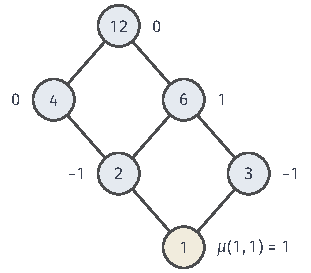
\includegraphics[width=52.613mm]{figures/01-basic-mathematics/04-graphs/tikz/c4-mobius-divisor-poset/figure.pdf}
  \caption{$12$的正因数在整除关系下的偏序，连线连接直接相邻的两个因数，下方整除上方。节点旁的数是$\mu(1,x)$，由$\mu(1,1)=1$（黄色节点）自下而上递推得到。链$1\mid2\mid4$上$\mu(1,4)=0$，与子集格同形的区间$\{1,2,3,6\}$上$\mu(1,6)=1$。}
  \label{fig:graph-setfn-mobius-divisors}
\end{figure}

% 第4章第4节：基数约束下的子集选择（基数约束与选择目标；边际增益贪心算法；贪心保证与适用范围）。

\section{基数约束下的子集选择}
\label{sec:graph-cardinality-selection}

回到传感器。预算只允许安装$k$个传感器时，应当选哪几个？本节先把目标、可行集合和函数的给定方式写清楚，再介绍逐轮加入边际增益最大元素的贪心算法，最后证明目标单调且次模时这种算法的近似保证，并用反例说明撤去条件后保证怎样失效。

\subsection{基数约束与选择目标}
\label{sec:graph-setfn-cardinality-problem}

设$V$是$n$元底集，$F$是$V$上的集合函数，整数$k$满足$0\leq k\leq n$。要求的是
\begin{equation}
  \max_{S\subseteq V,\ |S|\leq k}F(S).
  \label{eq:graph-setfn-cardinality-problem}
\end{equation}
“至多选$k$个”称为\term{基数约束}（cardinality constraint）。函数$F$通过求值规则给出：算法可以对任意子集询问$F$的值，每次询问计一次求值。

对单调函数，“至多$k$个”与“恰好$k$个”给出同样的最优值。若某个最优集合不足$k$个元素，任意补入元素使它恰有$k$个，由单调性函数值不会下降，补足后的集合仍是最优的。非单调函数不能这样处理：补入的元素可能降低目标值，所以“至多”与“恰好”是两个不同的问题。

\paragraph{枚举作为基准}
小底集可以枚举全部可行子集。在传感器实例中取$k=2$，可行子集有$\binom40+\binom41+\binom42=11$个。逐个计算覆盖量，最优值是$16$，最优集合唯一，为$\{b,c\}$；单元素中最好的是$\{a\}$，覆盖$10$格。一般地，最优值是唯一的，最优集合却可能有多个并列；$k=3$时，$\{b,c\}$、$\{a,b,c\}$、$\{b,c,d\}$都覆盖全部$16$个格子，按“至多$3$个”的约束三者都是最优集合。

枚举在规模稍大时就不可行。即使一次求值很便宜，$n=100$、$k=10$时，仅恰有$10$个元素的子集就有$\binom{100}{10}\approx1.7\times10^{13}$个。我们需要一种只看少量子集、利用边际增益结构逐步构造解的方法。

\subsection{边际增益贪心算法}
\label{sec:graph-setfn-greedy}

最自然的逐步构造是：每一轮在尚未选中的元素里，挑当前增益最大的那个加入。这里的“当前”很关键，增益要相对于已经选好的集合重新计算。

\begin{algorithm}[基数约束下的边际增益贪心]
\label{alg:graph-setfn-greedy}
输入：有限底集$V$（元素已编号），整数$0\leq k\leq|V|$，单调非减集合函数$F$的求值规则。输出：至多含$k$个元素的集合。状态：当前已选集合$S_{t-1}$及其函数值，本轮各候选元素的增益。
\begin{enumerate}
  \item 令$S_0=\varnothing$，记录$F(S_0)$。
  \item 对$t=1,\ldots,k$：对每个$v\in V\setminus S_{t-1}$，求值$F(S_{t-1}\cup\{v\})$，得到$\Delta(v\mid S_{t-1})$；取增益最大的$v_t$，增益相同时取编号最小者；令$S_t=S_{t-1}\cup\{v_t\}$。
  \item 输出$S_k$。
\end{enumerate}
\end{algorithm}

由于假设$F$单调，每一轮的增益都非负，加入元素不会使目标下降，算法总是选满$k$个。平局规则必须事先规定，否则同一输入可能得到不同输出，结果无法复核。

\paragraph{逐轮轨迹}
在传感器实例上取$k=2$，按字母顺序编号。图~\ref{fig:graph-setfn-greedy-rounds}列出每一轮的候选增益。第$1$轮从空集出发，增益就是各传感器单独的覆盖量：$a$为$10$，$b,c$各为$8$，$d$为$1$，选$a$。第$2$轮相对于$\{a\}$重新计算：$b$只补上第$1$列的$2$格，$c$补上第$7$、$8$列的$4$格，$d$补上$1$格，选$c$。贪心结果是$\{a,c\}$，覆盖$14$格；枚举得到的最优集合是$\{b,c\}$，覆盖$16$格。

\begin{figure}[!htb]
  \centering
  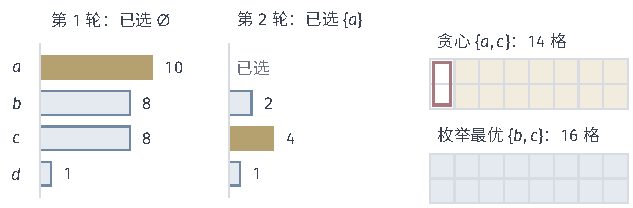
\includegraphics[width=107.177mm]{figures/01-basic-mathematics/04-graphs/tikz/c4-greedy-rounds-vs-optimum/figure.pdf}
  \caption{传感器实例上$k=2$的边际增益贪心。左侧两栏是两轮中各候选元素的当前增益，黄色条为该轮选中的元素；第$2$轮的增益相对于已选的$\{a\}$计算。右侧比较两个覆盖结果：贪心集合$\{a,c\}$（黄色）漏掉第$1$列两格（红框），枚举最优集合$\{b,c\}$（蓝色）覆盖全部$16$格。}
  \label{fig:graph-setfn-greedy-rounds}
\end{figure}

这条轨迹也说明为什么不能只按初始增益排序一次。初始增益的次序是$a$，然后$b,c$并列；按编号取前两个得到$\{a,b\}$，只覆盖$12$格。第$2$轮重新计算后，$b$的增益从$8$降到$2$，$c$的增益从$8$降到$4$，排序已经改变。

\paragraph{求值次数与缓存}
第$t$轮要对$n-t+1$个未选元素各求值一次，总共
\[
  \sum_{t=1}^{k}(n-t+1)\leq nk
\]
次求值，再加上开始时的一次$F(\varnothing)$。传感器实例$n=4$、$k=2$，共$4+3=7$次。若一次求值的代价为$\tau$（例如覆盖量需要合并若干覆盖范围），总代价是$O(nk\tau)$。

对次模函数，可以缓存上一轮算出的增益来减少求值。由式~\eqref{eq:graph-setfn-diminishing-returns}，已选集合变大后，每个元素的增益只会变小，所以旧增益是新增益的上界。每轮把候选元素按缓存值排序，只重新计算排在最前的元素；若它的新增益仍不小于其余元素的缓存值，它就是本轮增益最大者，其余元素不必重算。这种做法的正确性依赖次模性；对一般函数，旧增益不是上界，必须每轮全部重新计算。

\subsection{贪心保证与适用范围}
\label{sec:graph-setfn-greedy-guarantee}

贪心在传感器实例上没有找到最优解，但$14$与$16$相差不多。下面的定理说明这不是巧合：对归一化、单调、次模的目标，贪心值总能达到最优值的一个固定比例。

\begin{theorem}[贪心的近似保证]
\label{thm:graph-setfn-greedy-guarantee}
设$F$是有限底集$V$上的集合函数，满足$F(\varnothing)=0$、单调非减且次模；整数$1\leq k\leq|V|$。记$\mathrm{OPT}$为问题~\eqref{eq:graph-setfn-cardinality-problem}的最优值，$S_\ell$为算法~\ref{alg:graph-setfn-greedy}执行$\ell$轮后的集合（$0\leq\ell\leq k$）。则
\[
  F(S_\ell)\geq\Bigl(1-\bigl(1-\tfrac1k\bigr)^{\ell}\Bigr)\mathrm{OPT}.
\]
特别地，$F(S_k)\geq\bigl(1-(1-1/k)^k\bigr)\mathrm{OPT}\geq(1-e^{-1})\mathrm{OPT}$。
\end{theorem}

\begin{proof}
固定一个最优集合$O$，$|O|\leq k$，$F(O)=\mathrm{OPT}$。考察第$t$轮开始时的集合$S_{t-1}$（$1\leq t\leq k$），先用次模性把它与最优值的差距上界为若干个边际增益之和。把$O\setminus S_{t-1}$中的元素排成$o_1,\ldots,o_r$，由单调性和式~\eqref{eq:graph-setfn-telescoping}，
\[
  \mathrm{OPT}=F(O)\leq F(O\cup S_{t-1})
  =F(S_{t-1})+\sum_{j=1}^{r}\Delta\bigl(o_j\mid S_{t-1}\cup\{o_1,\ldots,o_{j-1}\}\bigr).
\]
每个$o_j$都不在$S_{t-1}\cup\{o_1,\ldots,o_{j-1}\}$中，由式~\eqref{eq:graph-setfn-diminishing-returns}，第$j$项不超过$\Delta(o_j\mid S_{t-1})$。而贪心在第$t$轮选的是增益最大的元素，所以$\Delta(o_j\mid S_{t-1})\leq\Delta(v_t\mid S_{t-1})=F(S_t)-F(S_{t-1})$。又$r\leq|O|\leq k$，且每一项增益非负，于是
\[
  \mathrm{OPT}-F(S_{t-1})\leq k\bigl(F(S_t)-F(S_{t-1})\bigr).
\]
这一步说的是：最优集合至多$k$个元素，它们合起来能补上的差距，至少有$1/k$能被当前最好的单个元素补上。

记差距$\delta_t=\mathrm{OPT}-F(S_t)$。上式可写成$\delta_{t-1}\leq k(\delta_{t-1}-\delta_t)$，即
\[
  \delta_t\leq\Bigl(1-\frac1k\Bigr)\delta_{t-1},\qquad t=1,\ldots,k.
\]
由$F(\varnothing)=0$得$\delta_0=\mathrm{OPT}$，连续使用$\ell$次得$\delta_\ell\leq(1-1/k)^\ell\,\mathrm{OPT}$，移项即为所求。

最后比较$(1-1/k)^k$与$e^{-1}$。函数$\psi(x)=e^{-x}-(1-x)$满足$\psi(0)=0$，导数$\psi'(x)=1-e^{-x}$在$x>0$时为正，所以$\psi$在$[0,+\infty)$上单调递增（第~\ref{sec:ru-monotonicity-convexity}节），从而$0\leq1-x\leq e^{-x}$对$0\leq x\leq1$成立。取$x=1/k$再求$k$次幂，得到$(1-1/k)^k\leq e^{-1}$。
\end{proof}

几个条件各有作用。归一化保证差距从$\mathrm{OPT}$开始；若$F(\varnothing)\neq0$，比例式会因为一个常数而失去意义。单调性用在$F(O)\leq F(O\cup S_{t-1})$和增益非负两处，次模性用在把$O$中元素的增益统一换成相对于$S_{t-1}$的增益。$k=1$时界为$1$，贪心选出的就是最好的单元素；$k=2$时界为$3/4$，传感器实例中$14\geq\frac34\times16=12$，与定理一致。$1-e^{-1}\approx0.632$是对一切$k$都成立的下界。

\paragraph{撤去次模性}
图~\ref{fig:graph-setfn-property-counterexamples}(a)的函数$F(S)=\max\{3\,\mathbb I\{\{1,2\}\subseteq S\},\mathbb I\{3\in S\}\}$单调、归一化，但不是次模的。取$k=2$：第$1$轮三个增益依次为$0,0,1$，选$3$；第$2$轮相对于$\{3\}$，加入$1$或$2$的增益都是$0$，按编号选$1$，得到$F(\{1,3\})=1$。最优集合是$\{1,2\}$，$\mathrm{OPT}=3$。元素$1,2$只有同时选中才有价值，每一轮单独看它们的增益都是零，贪心永远看不到这个互补组合。把$3$换成任意大的$M$，比例$1/M$可以任意小，所以没有次模性就没有固定比例的保证。

\paragraph{撤去单调性}
图~\ref{fig:graph-setfn-property-counterexamples}(b)的单边割权是次模的，但不单调。取$k=2$并按算法~\ref{alg:graph-setfn-greedy}强制选满：第$1$轮选$1$（增益$1$），第$2$轮只剩$2$，增益为$-1$，仍须加入，结果$\operatorname{cut}(\{1,2\})=0$，而至多选两个时的最优值是$1$。在增益为负时停止可以避免这个例子中的损失，但对一般的非单调次模函数，这样修改后的贪心仍没有定理~\ref{thm:graph-setfn-greedy-guarantee}那样的保证，需要另外的算法与分析，本节不展开。

因此，定理~\ref{thm:graph-setfn-greedy-guarantee}只适用于本节规定的问题：在基数约束下最大化归一化、单调、次模的集合函数。它给出的是近似比例，不是精确最优性；目标、约束或函数性质改变时，都需要重新论证。

% 第4章第5节：预算约束下的子集选择（预算约束选择问题；单位成本边际收益法；方法的局限与结果检查）。

\section{预算约束下的子集选择}
\label{sec:graph-budget-selection}

基数约束让每个元素占用一个名额。实际中不同传感器的价格不同，限制的往往是总花费而不是个数。本节说明换成预算约束后，可行集合、选择依据和性能分析各自怎样改变。主线是一种简单可算的逐轮规则，重点放在它的执行过程与失效边界，而不是把上一节的保证直接搬过来。

\subsection{预算约束选择问题}
\label{sec:graph-setfn-budget-problem}

给每个元素$v\in V$指定成本$c_v$，再给定总预算$B\geq0$。要求的是
\begin{equation}
  \max_{S\subseteq V}\ F(S)\qquad\text{满足}\quad\sum_{v\in S}c_v\leq B.
  \label{eq:graph-setfn-budget-problem}
\end{equation}
满足成本条件的子集称为预算可行的，这一条件称为\term{预算约束}（budget constraint）。目标函数$F$与上一节相同，改变的只是允许的子集。所有成本都取$1$、预算取$k$时，预算约束就是基数约束，所以本节的问题是上一节的推广。

成本可能为零的元素需要先单独处理。零成本元素不占预算，若$F$单调，把它们全部加入不会降低目标，可以在开始时一次放进集合；若$F$不单调，它们是否值得加入要看增益的正负。以下设所有成本为正。另外，成本超过$B$的元素不可能出现在任何可行集合中，可以预先删去。

\paragraph{两种约束下的可行集合}
在传感器实例中取成本$c_a=4$、$c_b=3$、$c_c=4$、$c_d=1$，预算$B=7$。预算可行的子集共有$10$个：空集、四个单元素集，以及$\{a,b\}$（成本$7$）、$\{a,d\}$（$5$）、$\{b,c\}$（$7$）、$\{b,d\}$（$4$）、$\{c,d\}$（$5$）；三元及以上的子集成本都超过$7$。枚举得最优集合为$\{b,c\}$，覆盖$16$格。与$k=2$的基数约束相比，$\{a,c\}$成本为$8$，现在不可行了；而$\{a,b\}$在两种约束下都可行。选择的个数不再直接决定资源消耗，每次加入元素前都要检查剩余预算。

\subsection{单位成本边际收益法}
\label{sec:graph-setfn-ratio-greedy}

把上一节的贪心原样搬过来，就是每轮在付得起的元素里选增益最大的。这样做会偏爱昂贵的元素：一个元素增益大，可能只是因为它贵。更合理的比较是每单位成本带来多少增益。

\begin{algorithm}[预算约束下的单位成本贪心]
\label{alg:graph-setfn-ratio-greedy}
输入：有限底集$V$（元素已编号），正成本$c_v$，预算$B\geq0$，单调非减集合函数$F$的求值规则。输出：预算可行的集合。状态：已选集合$S$，剩余预算$R=B-\sum_{v\in S}c_v$，本轮候选元素的增益。
\begin{enumerate}
  \item 令$S=\varnothing$，$R=B$。
  \item 记候选集合$Q=\{v\in V\setminus S:c_v\leq R\}$。若$Q$为空，停止。
  \item 对每个$v\in Q$计算$\Delta(v\mid S)$。若这些增益全为零，停止；否则取比值$\Delta(v\mid S)/c_v$最大的$v$，比值相同时取编号最小者。
  \item 令$S\leftarrow S\cup\{v\}$，$R\leftarrow R-c_v$，回到第2步。
\end{enumerate}
\end{algorithm}

每轮至少加入一个元素，所以算法至多执行$n$轮，求值次数不超过$n+(n-1)+\cdots+1=n(n+1)/2$。停止时有两种原因：没有付得起的元素，或者付得起的元素都不再增加覆盖。

\paragraph{两种规则的对照}
图~\ref{fig:graph-setfn-budget-rule-comparison}在$B=7$的实例上比较“总增益最大”与“单位成本增益最大”两种规则。按总增益，第$1$轮选$a$（增益$10$），剩余预算$3$；第$2$轮付得起的有$b$（增益$2$）和$d$（增益$1$），$c$的成本$4$超出剩余预算，选$b$，剩余预算$0$，停止，覆盖$12$格。按单位成本，第$1$轮的比值为$a:10/4=2.5$，$b:8/3\approx2.67$，$c:8/4=2$，$d:1/1=1$，选$b$，剩余预算$4$；第$2$轮相对于$\{b\}$，$a$的增益为$4$（第$5$、$6$列），比值$1$，$c$的增益为$8$，比值$2$，$d$的增益为$0$，选$c$，剩余预算$0$，停止，覆盖$16$格，恰为枚举最优值。

\begin{figure}[!htb]
  \centering
  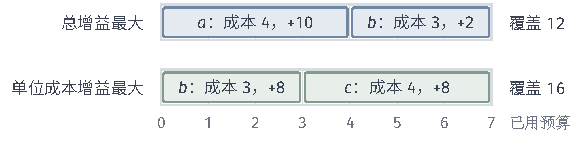
\includegraphics[width=98.538mm]{figures/01-basic-mathematics/04-graphs/tikz/c4-budget-rule-comparison/figure.pdf}
  \caption{预算$B=7$下两种逐轮规则的选择结果（成本$c_a=4$、$c_b=3$、$c_c=4$、$c_d=1$）。每条横条代表$7$个单位的预算，色块的宽度是所选元素的成本，块内写出选择时的增益。按总增益先选昂贵的$a$，剩余预算只够再选增益$2$的$b$，覆盖$12$格；按单位成本先选$b$，再选$c$，覆盖$16$格。}
  \label{fig:graph-setfn-budget-rule-comparison}
\end{figure}

\paragraph{与最佳单元素比较}
单位成本规则也有自己的偏差：它可能先选几个便宜的小元素，把预算切碎，使一个昂贵但价值很高的元素再也放不进去。一种简单的补救是在算法结束后，再计算每个可行单元素的值$F(\{v\})$（$c_v\leq B$），输出$S$与最佳单元素中函数值较大的一个。这只需另外$n$次求值。在$B=7$的实例中，最佳单元素是$\{a\}$，覆盖$10$格，小于$16$，输出仍是$\{b,c\}$。这一检查只是一个具体策略；本节没有给出它的分析，因此不附加一般的近似比例。

\subsection{方法的局限与结果检查}
\label{sec:graph-setfn-budget-limits}

单位成本规则在上面的实例中表现很好，但下面的例子说明它本身没有任何固定比例的保证。

\begin{example}[比值规则的失效]
\label{ex:graph-setfn-ratio-failure}
底集$\{u,w\}$，预算$B=100$。$u$的成本为$1$、价值为$2$，$w$的成本为$100$、价值为$100$，目标取模函数$F(S)=\sum_{v\in S}(\text{价值})$。它单调，也是次模的。

比值规则第$1$轮比较$2/1=2$与$100/100=1$，选$u$；剩余预算$99<100$，$w$付不起，算法停止，得$F(\{u\})=2$。最优选择是$\{w\}$，$F=100$。见图~\ref{fig:graph-setfn-budget-ratio-failure}。把$w$的成本、价值与预算同时换成任意大的$M$，比值规则仍先选$u$，得到$2$而最优值为$M$，比例$2/M$可以任意小。
\end{example}

\begin{figure}[!htb]
  \centering
  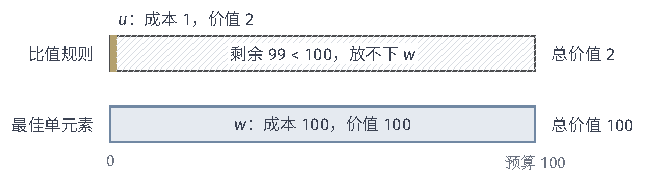
\includegraphics[width=109.146mm]{figures/01-basic-mathematics/04-graphs/tikz/c4-budget-ratio-failure/figure.pdf}
  \caption{比值规则的失效例。横条长度代表预算$100$。上行：比值规则先选单位价值较高的$u$（黄色，成本$1$，为便于观察略加宽），剩余$99$个单位（斜线）放不下成本$100$的$w$，总价值$2$。下行：最佳单元素$w$恰好用满预算，总价值$100$。}
  \label{fig:graph-setfn-budget-ratio-failure}
\end{figure}

这个例子的目标是模函数，从而单调且次模，可见即使目标满足上一节定理的全部函数条件，原始比值规则也不能继承那里的保证：预算约束改变了可行集合的结构，证明中“最优集合至多$k$个元素”这一步不再有对应物。上一小节的最佳单元素比较能修复这个例子，因为它会发现$\{w\}$；但修复一个例子不构成一般保证。具有严格保证的预算选择算法需要另外的枚举或修正机制，并要给出相应的证明，本书不展开，也不应把它们与这里的简单规则混为一谈。

\paragraph{结果检查}
小实例可以直接枚举全部预算可行子集，核对三件事：输出集合的总成本不超过预算，输出的函数值计算无误，以及它与枚举最优值的差距。上面$B=7$的实例只有$10$个可行子集，比值规则的结果$\{b,c\}$与枚举最优一致，总增益规则的结果$\{a,b\}$差$4$格。大实例无法枚举时，至少应报告所用预算与剩余预算、最终目标值、最佳单元素的值，以及总求值次数和每次求值的代价。最佳单元素给出一个必须超过的基准；若逐轮规则的结果不如它，往往就是出现了示例~\ref{ex:graph-setfn-ratio-failure}那样预算被小元素切碎的情形。

% 第4章第6节：成对二值函数的最小化（成对二值最小化问题；次模条件与割表示；最小割求解与解的恢复）。

\section{成对二值函数的最小化}
\label{sec:graph-pairwise-binary-cut}

前两节在约束下最大化一般的集合函数，只能得到近似解。本节换一个方向：目标是最小化，没有基数或预算约束，但函数具有特殊的结构，即由只涉及单个元素的一元项和只涉及两个元素的成对项相加而成。利用子集与二值向量的对应，我们把这样的目标在一定条件下表示为割的容量，再调用第~\ref{sec:graph-max-flow}节的最小割，求出精确的最优解。

\subsection{成对二值最小化问题}
\label{sec:graph-setfn-pairwise-problem}

给底集$V$的每个元素$i$一个二值变量$x_i\in\{0,1\}$，$x_i=1$表示选中$i$，于是配置$\bm x\in\{0,1\}^V$就是第~\ref{sec:graph-setfn-binary-vectors}节的指示向量。元素之间的交互用无向图$\mathcal G=(V,E)$记录：只有$\{i,j\}\in E$的两个元素之间有成对项。目标是
\begin{equation}
  \min_{\bm x\in\{0,1\}^V}J(\bm x),\qquad
  J(\bm x)=\sum_{i\in V}\phi_i(x_i)+\sum_{\{i,j\}\in E}\phi_{i,j}(x_i,x_j).
  \label{eq:graph-setfn-pairwise-objective}
\end{equation}
\term{一元项}$\phi_i$给出元素$i$两种状态各自的成本，只有两个数$\phi_i(0),\phi_i(1)$；\term{成对项}$\phi_{i,j}$给出$i,j$四种联合状态的成本，例如两者取值不同时的不一致代价，或两者同时选中的配合收益（以负成本表示）。为了让$\phi_{i,j}(a,b)$的含义确定，对每条边固定一个次序，约定$a$是$x_i$、$b$是$x_j$的值。本节只考虑有限实值成本。

通过$S=\{i:x_i=1\}$，$J$也是$V$上的集合函数。但并不是每个集合函数都能写成式~\eqref{eq:graph-setfn-pairwise-objective}的形式：例如只在三个元素同时选中时才产生的成本，不能拆成两两之间的成对项。本节的方法只适用于已经具有这种一元加成对结构的目标。

\paragraph{逐点选择为什么不够}
取两个变量，$\phi_1(0)=0$、$\phi_1(1)=1$，$\phi_2(0)=2$、$\phi_2(1)=0$，成对项为
\[
  \phi_{1,2}(0,0)=0,\quad\phi_{1,2}(0,1)=3,\quad\phi_{1,2}(1,0)=5,\quad\phi_{1,2}(1,1)=0.
\]
图~\ref{fig:graph-setfn-pairwise-config-table}列出四种配置的成本。若只看一元项，元素$1$偏好$0$，元素$2$偏好$1$，逐点选择得到$(0,1)$，成本$0+0+3=3$。但成对项惩罚两者取值不同，整体最优是$(1,1)$，成本$1+0+0=1$：让元素$1$放弃自己的偏好只多付$1$，却省下了$3$的不一致代价。

\begin{figure}[!htb]
  \centering
  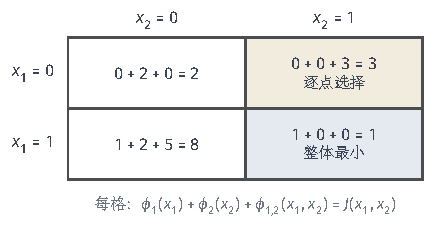
\includegraphics[width=72.383mm]{figures/01-basic-mathematics/04-graphs/tikz/c4-pairwise-config-table/figure.pdf}
  \caption{两变量成对二值函数的四种配置。行是$x_1$，列是$x_2$，每格依次写出$\phi_1(x_1)$、$\phi_2(x_2)$、$\phi_{1,2}(x_1,x_2)$与总成本$J$。逐点按一元项选择得到黄色格$(0,1)$，成本$3$；整体最小是蓝色格$(1,1)$，成本$1$。}
  \label{fig:graph-setfn-pairwise-config-table}
\end{figure}

两个变量可以枚举，$n$个变量则有$2^n$种配置。下面把四种配置的成本同时编码进一个网络的割容量，使枚举变成一次最小割计算。

\subsection{次模条件与割表示}
\label{sec:graph-setfn-cut-representation}

割容量只能累加非负的弧容量，因此能否编码取决于成对项的形状。关键条件是对每条边$\{i,j\}\in E$成立
\begin{equation}
  \phi_{i,j}(0,0)+\phi_{i,j}(1,1)\leq\phi_{i,j}(0,1)+\phi_{i,j}(1,0).
  \label{eq:graph-setfn-pairwise-submodular}
\end{equation}
它正是两元素底集$\{i,j\}$上的次模不等式：把$\phi_{i,j}$看成$\{i,j\}$上的集合函数，在式~\eqref{eq:graph-setfn-submodular-inequality}中取$X=\{i\}$、$Y=\{j\}$，左边$F(X)+F(Y)$对应$\phi_{i,j}(1,0)+\phi_{i,j}(0,1)$，右边$F(X\cup Y)+F(X\cap Y)$对应$\phi_{i,j}(1,1)+\phi_{i,j}(0,0)$。一元项是模函数，若每个成对项都满足式~\eqref{eq:graph-setfn-pairwise-submodular}，则$J$作为集合函数是次模的。上面的例子中$0+0\leq3+5$，条件成立。

\paragraph{成对项的分解}
条件~\eqref{eq:graph-setfn-pairwise-submodular}允许把一个成对项拆成常数、两个一元的线性部分和一个非负的不一致惩罚。

\begin{lemma}[成对项的分解]
\label{lem:graph-setfn-pairwise-decomposition}
设$\phi_{i,j}$满足式~\eqref{eq:graph-setfn-pairwise-submodular}，简记$p_{a,b}=\phi_{i,j}(a,b)$，令
\[
  \begin{gathered}
  w_{i,j}=\frac{p_{0,1}+p_{1,0}-p_{0,0}-p_{1,1}}{2},\\
  \alpha_i=p_{1,0}-p_{0,0}-w_{i,j},\qquad
  \alpha_j=p_{0,1}-p_{0,0}-w_{i,j}.
  \end{gathered}
\]
则$w_{i,j}\geq0$，并且对四种配置都有
\begin{equation}
  \phi_{i,j}(x_i,x_j)=p_{0,0}+\alpha_ix_i+\alpha_jx_j+w_{i,j}\,|x_i-x_j|.
  \label{eq:graph-setfn-pairwise-decomposition}
\end{equation}
\end{lemma}

\begin{proof}
$w_{i,j}\geq0$就是式~\eqref{eq:graph-setfn-pairwise-submodular}移项除以$2$。逐个代入四种配置核对右边：$(0,0)$时为$p_{0,0}$；$(1,0)$时为$p_{0,0}+\alpha_i+w_{i,j}=p_{1,0}$；$(0,1)$时为$p_{0,0}+\alpha_j+w_{i,j}=p_{0,1}$；$(1,1)$时为$p_{0,0}+\alpha_i+\alpha_j=p_{1,0}+p_{0,1}-p_{0,0}-2w_{i,j}=p_{1,1}$，最后一步代入$w_{i,j}$的定义。
\end{proof}

在例子中，$w_{1,2}=(3+5-0-0)/2=4$，$\alpha_1=5-0-4=1$，$\alpha_2=3-0-4=-1$。

\paragraph{一元项的合并与移位}
对每条边作上述分解，把常数$\phi_{i,j}(0,0)$累加起来，把线性部分$\alpha_ix_i$、$\alpha_jx_j$并入相应元素的一元项。记合并后的一元项为$\psi_i$，即$\psi_i(0)=\phi_i(0)$，$\psi_i(1)=\phi_i(1)$加上与$i$关联的各边分解出的$\alpha_i$。$\psi_i$可能取负值，而容量必须非负，所以再令$m_i=\min\{\psi_i(0),\psi_i(1)\}$，$\tilde\psi_i=\psi_i-m_i$，两种状态的成本都减去同一个数，$\tilde\psi_i$的两个值非负且至少一个为零。移出的数另行累计成常数
\[
  K=\sum_{\{i,j\}\in E}\phi_{i,j}(0,0)+\sum_{i\in V}m_i .
\]
于是对每个配置都有
\begin{equation}
  J(\bm x)=K+\sum_{i\in V}\tilde\psi_i(x_i)+\sum_{\{i,j\}\in E}w_{i,j}\,|x_i-x_j|,
  \label{eq:graph-setfn-shifted-objective}
\end{equation}
右边除常数$K$外各项都非负。在例子中，$\psi_1=(0,\,1+1)=(0,2)$，$\psi_2=(2,\,0-1)=(2,-1)$；$m_1=0$，$m_2=-1$，所以$\tilde\psi_1=(0,2)$，$\tilde\psi_2=(3,0)$，$K=0+0+(-1)=-1$。

\paragraph{网络构造}
由式~\eqref{eq:graph-setfn-shifted-objective}构造有向网络：顶点为$V\cup\{s,t\}$；对每个$i\in V$，建弧$s\to i$，容量$\tilde\psi_i(1)$，以及弧$i\to t$，容量$\tilde\psi_i(0)$；对每条边$\{i,j\}\in E$，建方向相反的两条弧$i\to j$与$j\to i$，容量都是$w_{i,j}$。容量为零的弧可以省略。规定源侧的元素取$0$、汇侧的元素取$1$，即配置$\bm x$对应$s$--$t$割$(S_{\bm x},\bar S_{\bm x})$，其中$S_{\bm x}=\{s\}\cup\{i:x_i=0\}$。用最小割求解这类问题的方法常称为\term{图割}（graph cut）。

\begin{theorem}[成对二值函数的割表示]
\label{thm:graph-setfn-cut-representation}
设式~\eqref{eq:graph-setfn-pairwise-objective}中的成本都是有限实数，且每个成对项满足式~\eqref{eq:graph-setfn-pairwise-submodular}。则在上面构造的网络中，配置与$s$--$t$割一一对应，并且每个配置$\bm x$对应的割容量等于$J(\bm x)-K$。因此最小割对应的配置是$J$的最小点。
\end{theorem}

\begin{proof}
任一$s$--$t$割的源侧都含$s$、不含$t$，由$V$中哪些元素在源侧唯一确定，所以割与配置一一对应。割容量只累计从源侧指向汇侧的弧，逐类计算。若$x_i=0$，$i$在源侧，弧$i\to t$跨出，计入$\tilde\psi_i(0)$，弧$s\to i$两端都在源侧，不计入；若$x_i=1$，$i$在汇侧，弧$s\to i$跨出，计入$\tilde\psi_i(1)$，弧$i\to t$两端都在汇侧，不计入。两种情形合起来恰好计入$\tilde\psi_i(x_i)$。对边$\{i,j\}$，若$x_i=x_j$，两条弧都不跨越；若$x_i\neq x_j$，两条反向弧中恰有一条从源侧指向汇侧，计入一次$w_{i,j}$。合起来恰好计入$w_{i,j}|x_i-x_j|$。所以割容量等于式~\eqref{eq:graph-setfn-shifted-objective}右边去掉$K$，即$J(\bm x)-K$。$K$与配置无关，最小化割容量与最小化$J$是同一件事。
\end{proof}

在例子中，网络有弧$s\to1$（容量$2$）、$2\to t$（容量$3$）、$1\to2$与$2\to1$（容量都是$4$），弧$1\to t$与$s\to2$容量为零。表~\ref{tab:graph-setfn-cut-check}逐个核对四种配置：割容量都比$J$大$1$，即$-K$。

\begin{table}[!htb]
  \centering
  \begin{tabular}{cccc}
    \toprule
    配置$\bm x$ & 源侧 & 跨出的正容量弧 & 割容量 / $J(\bm x)$ \\
    \midrule
    $(0,0)$ & $\{s,1,2\}$ & $2\to t$ & $3$ / $2$ \\
    $(0,1)$ & $\{s,1\}$ & $1\to2$ & $4$ / $3$ \\
    $(1,0)$ & $\{s,2\}$ & $s\to1$，$2\to t$，$2\to1$ & $9$ / $8$ \\
    $(1,1)$ & $\{s\}$ & $s\to1$ & $2$ / $1$ \\
    \bottomrule
  \end{tabular}
  \caption{两变量例子中四种配置的割容量与原目标值。源侧元素取$0$、汇侧元素取$1$；每行割容量都等于$J(\bm x)+1$，相差的常数是$-K=1$，所以割容量最小的$(1,1)$也是$J$的最小点。}
  \label{tab:graph-setfn-cut-check}
\end{table}

\paragraph{条件不成立时}
若某个成对项违反式~\eqref{eq:graph-setfn-pairwise-submodular}，引理给出的$w_{i,j}$为负，网络中就会出现负容量的弧。第~\ref{sec:graph-max-flow}节的流值与割容量的关系建立在非负容量之上，负容量时不能直接使用。例如奖励两个变量取值不同的成对项$\phi_{i,j}(0,1)=\phi_{i,j}(1,0)=0$、$\phi_{i,j}(0,0)=\phi_{i,j}(1,1)=1$就违反条件，这时的最小化一般不能化为一次最小割。

\subsection{最小割求解与解的恢复}
\label{sec:graph-setfn-cut-solving}

\paragraph{求解步骤}
构造网络后，用第~\ref{sec:graph-max-flow}节的Edmonds--Karp算法求最大流。算法停止时，残量网络中从$s$可达的顶点集合是一个最小割的源侧；把其中的元素标为$0$，其余元素标为$1$，就得到最优配置$\hat{\bm x}$。结果可以独立核对：直接按式~\eqref{eq:graph-setfn-pairwise-objective}计算$J(\hat{\bm x})$，它应等于最大流值加$K$。由于最大流值等于最小割容量，这个等式同时证明了$\hat{\bm x}$的最优性，而不必相信算法实现本身。

\paragraph{两变量例子的求解}
网络中从$s$到$t$只有一条正容量路径$s\to1\to2\to t$，瓶颈为$\min\{2,4,3\}=2$。沿它增广$2$个单位后，$s\to1$的正向残量为零，$s\to2$本来容量为零，所以残量网络中从$s$出发哪里也到不了，可达集合是$\{s\}$。最小割容量$2$等于流值，两个元素都在汇侧，得到$\hat{\bm x}=(1,1)$。代回原目标，$J(1,1)=1+0+0=1=2+K$，与图~\ref{fig:graph-setfn-pairwise-config-table}中的枚举结果一致。图~\ref{fig:graph-setfn-st-cut-construction}把这个最小割与配置$(0,1)$对应的割并排比较。

\begin{figure}[!htb]
  \centering
  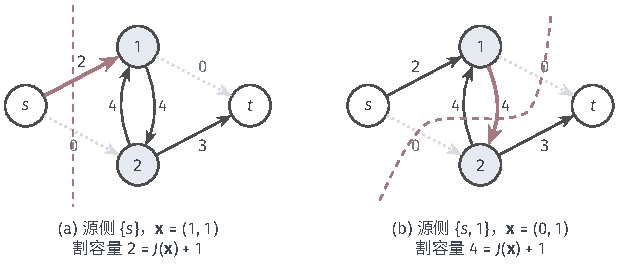
\includegraphics[width=104.687mm]{figures/01-basic-mathematics/04-graphs/tikz/c4-st-cut-construction/figure.pdf}
  \caption{两变量例子的$s$--$t$网络。弧旁数字是容量，灰色点线是容量为零的弧；红色虚线分开源侧与汇侧，红色粗弧是跨出割的正容量弧。源侧元素取$0$、汇侧元素取$1$。(a) 最小割，源侧$\{s\}$，只割断$s\to1$，容量$2$，对应$(1,1)$；(b) 源侧$\{s,1\}$，割断$1\to2$，容量$4$，对应逐点选择得到的$(0,1)$。两种情况的割容量都等于$J(\bm x)+1$。}
  \label{fig:graph-setfn-st-cut-construction}
\end{figure}

\paragraph{开销}
网络有$n+2$个顶点，弧数$a\leq2n+2m$，其中$m=|E|$；计算分解、合并一元项和建弧都只需扫描一遍元素与边，用时$O(n+m)$。主要开销在最大流：按第~\ref{sec:graph-max-flow}节的分析，Edmonds--Karp算法需要$O(na^2)$次算术与比较操作，代入$a=O(n+m)$即$O(n(n+m)^2)$。与枚举$2^n$种配置相比，这是多项式规模的计算。

\paragraph{与前两节的比较}
本节与前两节都在子集上做选择，但条件和结论不同。前两节在基数或预算约束下最大化单调次模函数，得到的是近似解，保证依赖单调性、次模性和约束的形式。本节最小化可以写成一元项加满足式~\eqref{eq:graph-setfn-pairwise-submodular}的成对项的函数，没有额外约束，得到的是精确解，依据是割表示。在本节的问题上再加“恰好选$k$个”这样的数量限制，割与配置的对应就不再保持约束；含三个及以上变量的高阶项、违反条件的成对项，以及每个变量有三种以上取值的问题，也都不能直接套用这个构造。一般次模函数的最小化另有专门的算法，超出本书范围。

% 第4章第7节：本章小结。

\section{本章小结}
\label{sec:graph-set-functions-summary}

本章从传感器覆盖出发，把对整组选择的评价写成有限底集上的集合函数。元素之间若互不影响，每个元素贡献一个固定的数，集合函数就是模函数；覆盖范围的重叠使边际增益随已选集合增大而递减，这就是次模性；部件之间的协同则产生相反方向的超模性。单调、模、次模各自约束不同的东西，覆盖量、割权和净收益说明它们可以以各种方式组合，判断时要回到边际增益或四个函数值的不等式逐项核对。子集累计与Möbius反演完成的是另一项任务：已知全部子集的累计值，按元素个数之差交替加减，恢复每个子集自身的贡献；它只依赖有限求和与包含关系，结果可以为负，计算开销随底集大小指数增长。

选择问题按目标方向与约束分别处理。在基数约束下最大化归一化、单调、次模的函数，逐轮加入当前增益最大的元素，所得值不低于最优值的$1-(1-1/k)^k$倍；撤去次模性，贪心会错过互补组合，撤去单调性，强制选满会降低目标。换成预算约束后，单位成本规则在传感器实例中找到了最优解，但在成本为$(1,2)$与$(100,100)$的例子中可以任意差，最佳单元素比较只修复个别失效。最小化由一元项和满足次模条件的成对项组成的函数时，目标可以表示为$s$--$t$网络的割容量，一次最小割给出精确解，并附带可以独立核对的证书。使用任何一种方法之前，都要同时写明目标方向、约束、单调性、次模性以及函数的表示结构。

第~\ref{sec:graph-pairwise-binary-cut}节的成功依赖两点：每个变量只有两种状态，成对项满足特定的不等式。许多问题两点都不满足，变量可以有更多取值，局部成本可以同时读取三个变量，或者直接禁止某些组合；但整体函数常常仍是许多局部项之和，每一项只读取少数变量。第~\ref{chap:graph-dynamic-programming}章从这里出发，研究怎样借助记录局部项读取关系的依赖图，把对全部配置的枚举化为沿图逐步传递的小规模表格计算。

